\begin{figure}[h]
\centering
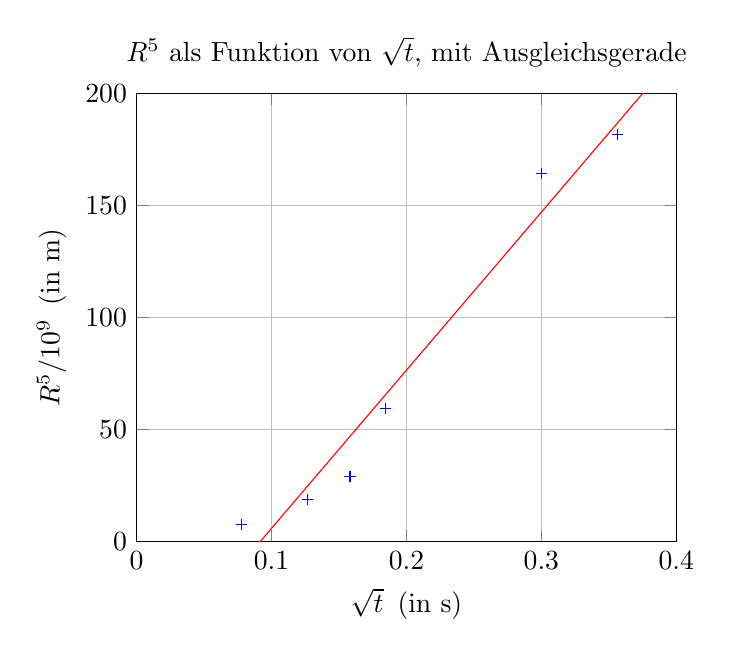
\begin{tikzpicture}
	\begin{axis}[xmin = 0, xmax = 0.4, ymin = 0, ymax = 200, grid = major, xlabel = {$\sqrt{t}~\left(\mathrm{in~s}\right)$}, ylabel = $R^5/10^{9}~\left(\mathrm{in~m}\right)$, title ={ $R^5$ als Funktion von $\sqrt{t}$, mit Ausgleichsgerade} ]

\addplot[blue, only marks, mark = +] coordinates
{(0.0774597, 7.73781) (0.158114, 29.0918) (0.126491, 18.949) (0.3, 
		164.131) (0.184391, 59.499) (0.356371, 181.577)};

\addplot[red] {-64.532+705.153*x};

	\end{axis}
\end{tikzpicture}
\end{figure}